\documentclass[a4paper,5pt]{amsbook}
%%%%%%%%%%%%%%%%%%%%%%%%%%%%%%%%%%%%%%%%%%%%%%%%%%%%%%%%%%%%%%%%%%%%%

\usepackage{booktabs}
\usepackage{graphicx}
\usepackage{multicol}
\usepackage{textcomp}
\usepackage{systeme}
\usepackage{amssymb}
\usepackage[]{amsmath}
\usepackage{subcaption}
\usepackage[inline]{enumitem}
\usepackage{gensymb}

%%%%%%%%%%%%%%%%%%%%%%%%%%%%%%%%%%%%%%%%%%%%%%%%%%%%%%%%%%%%%%

\newcommand{\sen}{\,\mbox{sen}}
\newcommand{\tg}{\,\mbox{tg}\,}
\newcommand{\cosec}{\,\mbox{cosec}\,}
\newcommand{\cotg}{\,\mbox{cotg}\,}
\newcommand{\tr}{\,\mbox{tr}\,}
\newcommand{\ds}{\displaystyle}
\newcommand{\ra}{\rightarrow}

%%%%%%%%%%%%%%%%%%%%%%%%%%%%%%%%%%%%%%%%%%%%%%%%%%%%%%%%%%%%%%%%%%%%%%%%

\setlength{\textwidth}{16cm} \setlength{\topmargin}{-1.7cm}
\setlength{\textheight}{25cm}
\setlength{\leftmargin}{1.2cm} \setlength{\rightmargin}{1.2cm}
\setlength{\oddsidemargin}{0cm}\setlength{\evensidemargin}{0cm}

%%%%%%%%%%%%%%%%%%%%%%%%%%%%%%%%%%%%%%%%%%%%%%%%%%%%%%%%%%%%%%%%%%%%%%%%

% \renewcommand{\baselinestretch}{1.6}
% \renewcommand{\thefootnote}{\fnsymbol{footnote}}
% \renewcommand{\theequation}{\thesection.\arabic{equation}}
% \setlength{\voffset}{-50pt}
% \numberwithin{equation}{chapter}

%%%%%%%%%%%%%%%%%%%%%%%%%%%%%%%%%%%%%%%%%%%%%%%%%%%%%%%%%%%%%%%%%%%%%%%

\begin{document}
\thispagestyle{empty}
\pagestyle{empty}
\begin{minipage}[h]{0.14\textwidth}
	
\includegraphics[scale=0.24]{../ufgd.png}
\end{minipage}
\begin{minipage}[h]{\textwidth}
\begin{tabular}{c}
{{\bf UNIVERSIDADE FEDERAL DA GRANDE DOURADOS}}\\
{{\bf C\'alculo Diferencial e Integral --- Lista 4}}\\
{{\bf Prof.\ Adriano Barbosa}}\\
\end{tabular}
\vspace{-0.45cm}
%
\end{minipage}

%------------------------

\vspace{1cm}
%%%%%%%%%%%%%%%%%%%%%%%%%%%%%%%%   formulario  inicio  %%%%%%%%%%%%%%%%%%%%%%%%%%%%%%%%
\begin{enumerate}
    \vspace{0.5cm}
    \item Se uma pedra for lan\c{c}ada para cima no planeta Marte com velocidade de
        $10$m/s, sua altura em metros $t$ segundos depois do lan\c{c}amento \'e dada
        por $y=10t-1,86t^2$.
        \begin{enumerate}
            \item Enconre a velocidade m\'edia da pedra nos intervalos abaixo:

                \begin{enumerate*}
                    \item $[1,\ 2]$
                        \hspace{0.2cm}
                        \hspace{0.2cm}
                    \item $[1,\ 1,5]$
                        \hspace{0.2cm}
                        \hspace{0.2cm}
                    \item $[1,\ 1,1]$
                        \hspace{0.2cm}
                        \hspace{0.2cm}
                    \item $[1,\ 1,01]$
                        \hspace{0.2cm}
                        \hspace{0.2cm}
                    \item $[1,\ 1,001]$
                \end{enumerate*}
            \item Estime a velocidade instant\^anea quando $t=1s$.
        \end{enumerate}

    \vspace{0.5cm}
    \item Para a fun\c{c}\~ao $h$ cujo gr\'afico \'e dado abaixo, determine os valores,
        quando poss\'{\i}vel.
        \begin{figure}[h]
            \centering
            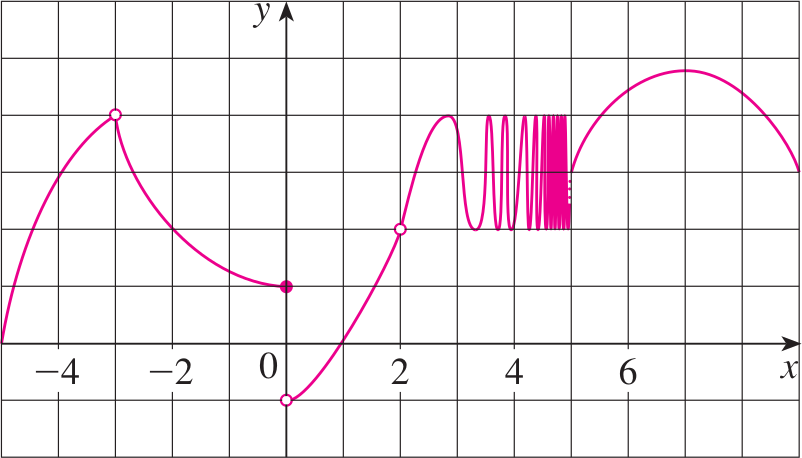
\includegraphics[width=0.5\textwidth]{lista-04-fig1.png}
        \end{figure}

        \noindent{}
        \begin{enumerate*}
            \item $\ds\lim_{x\ra -3^-} h(x)$
                \hspace{0.2cm}
                \hspace{0.2cm}
            \item $\ds\lim_{x\ra -3^+} h(x)$
                \hspace{0.2cm}
                \hspace{0.2cm}
            \item $\ds\lim_{x\ra -3} h(x)$
                \hspace{0.2cm}
                \hspace{0.2cm}
            \item $h(-3)$
                \hspace{0.2cm}
                \hspace{0.2cm}
            \item $\ds\lim_{x\ra 0^-} h(x)$
                \hspace{0.2cm}
                \hspace{0.2cm}
            \item $\ds\lim_{x\ra 0^+} h(x)$
                \hspace{0.2cm}
                \hspace{0.2cm}
            \item $\ds\lim_{x\ra 0} h(x)$
                \hspace{0.2cm}
                \hspace{0.2cm}
            \item $h(0)$
                \hspace{0.2cm}
                \hspace{0.2cm}
            \item $\ds\lim_{x\ra 5^-} h(x)$
                \hspace{0.2cm}
                \hspace{0.2cm}
            \item $\ds\lim_{x\ra 5^+} h(x)$
        \end{enumerate*}

    \vspace{0.5cm}
    \item Use a tabela de valores para estimar o valor dos limites abaixo.
        Utilize o computador para plotar os gr\'aficos e confirmar sua resposta
        graficamente.

        \begin{enumerate*}
            \item $\ds\lim_{x \ra 0} \frac{\sqrt{x+4}-2}{x}$
                \hspace{0.5cm}
                \hspace{0.5cm}
            \item $\ds\lim_{x \ra 0} \frac{\tan{3x}}{\tan{5x}}$
                \hspace{0.5cm}
                \hspace{0.5cm}
            \item $\ds\lim_{x \ra 1} \frac{x^6-1}{x^{10}-1}$
        \end{enumerate*}

    \vspace{0.5cm}
    \item Estime o valor de $\ds\lim_{x\rightarrow 0} \frac{\sen(x)}{x}$.

    \vspace{0.5cm}
    \item Dado que $\ds\lim_{x \ra 2} f(x)=4$, $\ds\lim_{x \ra 2} g(x)=-2$ e
        $\ds\lim_{x \ra 2} h(x)=0$, calcule os limites abaixo, caso existam.

        \noindent{}
        \begin{enumerate*}
            \item $\ds\lim_{x \ra 2} \left[f(x)+5g(x)\right]$
                \hspace{0.2cm}
                \hspace{0.2cm}
            \item $\ds\lim_{x \ra 2} {\left[g(x)\right]}^3$
                \hspace{0.2cm}
                \hspace{0.2cm}
            \item $\ds\lim_{x \ra 2} \sqrt{f(x)}$
                \hspace{0.2cm}
                \hspace{0.2cm}
            \item $\ds\lim_{x \ra 2} \frac{3f(x)}{g(x)}$
                \hspace{0.2cm}
                \hspace{0.2cm}
            \item $\ds\lim_{x \ra 2} \frac{g(x)}{h(x)}$
                \hspace{0.2cm}
                \hspace{0.2cm}
            \item $\ds\lim_{x \ra 2} \frac{g(x)h(x)}{f(x)}$
        \end{enumerate*}

    \vspace{0.5cm}
    \item Calcule os limites abaixo, caso existam:

        \noindent{}
        \begin{enumerate*}
            \item $\ds\lim_{x \ra 5} \frac{x^2-6x+5}{x-5}$
                \hspace{0.2cm}
                \hspace{0.2cm}
            \item $\ds\lim_{t \ra -3} \frac{t^2-9}{2t^2+7y+3}$
                \hspace{0.2cm}
                \hspace{0.2cm}
            \item $\ds\lim_{h \ra 0} \frac{\sqrt{9+h}-3}{h}$
                \hspace{0.2cm}
                \hspace{0.2cm}
            \item $\ds\lim_{t \ra 0} \frac{\sqrt{1+t}-\sqrt{1-t}}{t}$
                \hspace{0.2cm}
                \hspace{0.2cm}
            \item $\ds\lim_{x \ra 16} \frac{4-\sqrt{x}}{16x-x^2}$
        \end{enumerate*}

    \vspace{0.5cm}
    \item Se $4x-9\le f(x) \le x^2-4x+7$ para $x\ge 0$, calcule $\ds\lim_{x \ra 4} f(x)$.

    \vspace{0.5cm}
    \item Se $2x\le g(x)\le x^4-x^2+2$ para todo $x$, calcule $\ds\lim_{x \ra 1} g(x)$.
\end{enumerate}

\end{document}
